\chapter{Annex}


\begin{figure}
  \centering
  \subfigure[Constant Step Size Polar Coordinates]{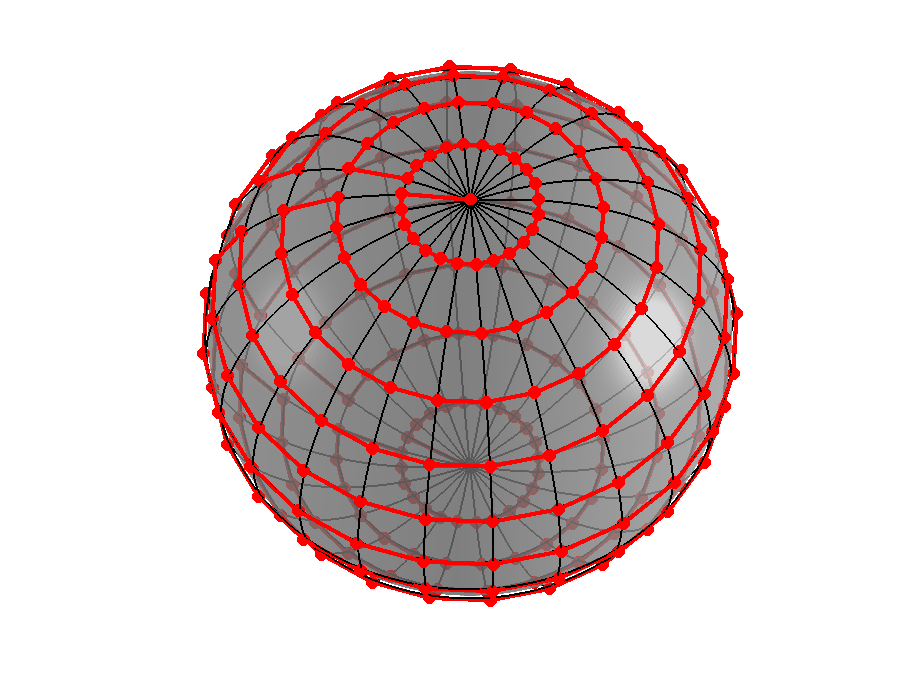
\includegraphics[width=0.49\textwidth]{Matlab/GridCoStPolar.eps}}
  \centering
  \subfigure[Constant Step Size Cartesian Coordinates]{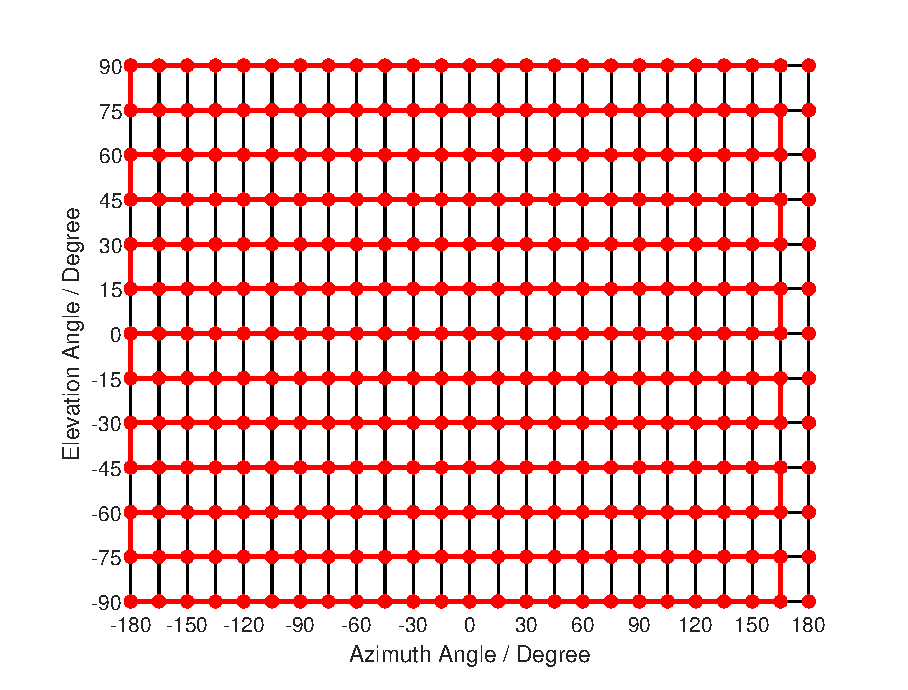
\includegraphics[width=0.49\textwidth]{Matlab/GridCoStCart.eps}}
  \centering
  \subfigure[Constant Step Size sinTF Polar Coordinates]{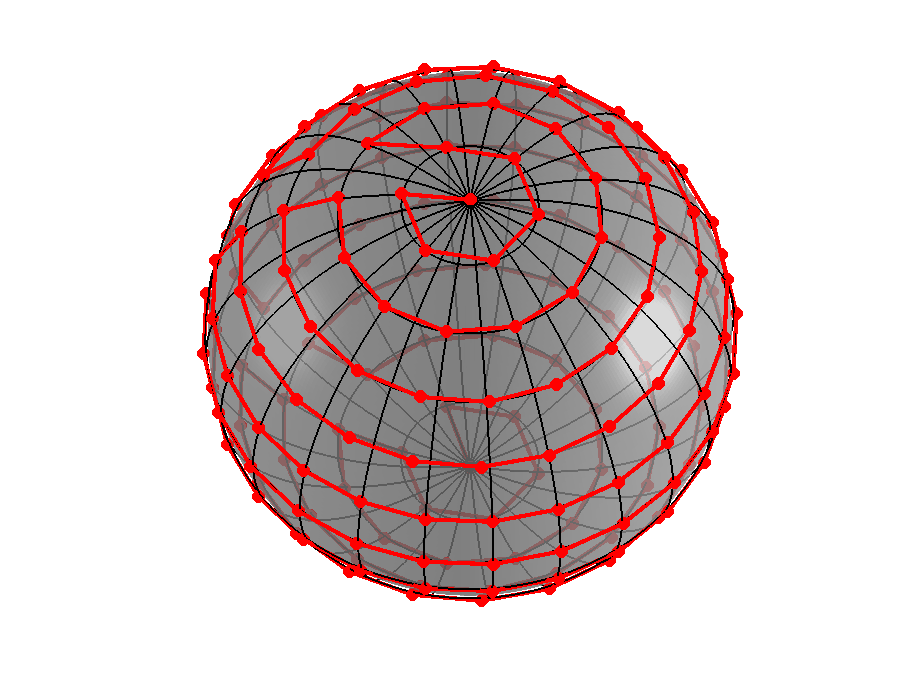
\includegraphics[width=0.49\textwidth]{Matlab/GridCoStSinPolar.eps}}
  \centering
  \subfigure[Constant Step Size sinTF Cartesian Coordinates]{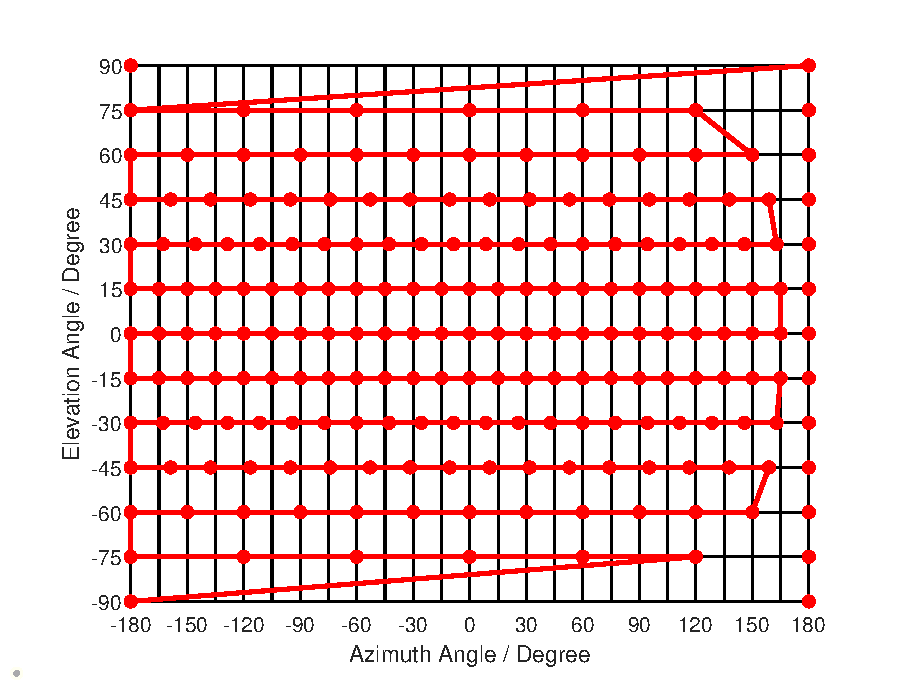
\includegraphics[width=0.49\textwidth]{Matlab/GridCoStSinCart.eps}}
  \centering
  \subfigure[Constant Density Polar Coordinates]{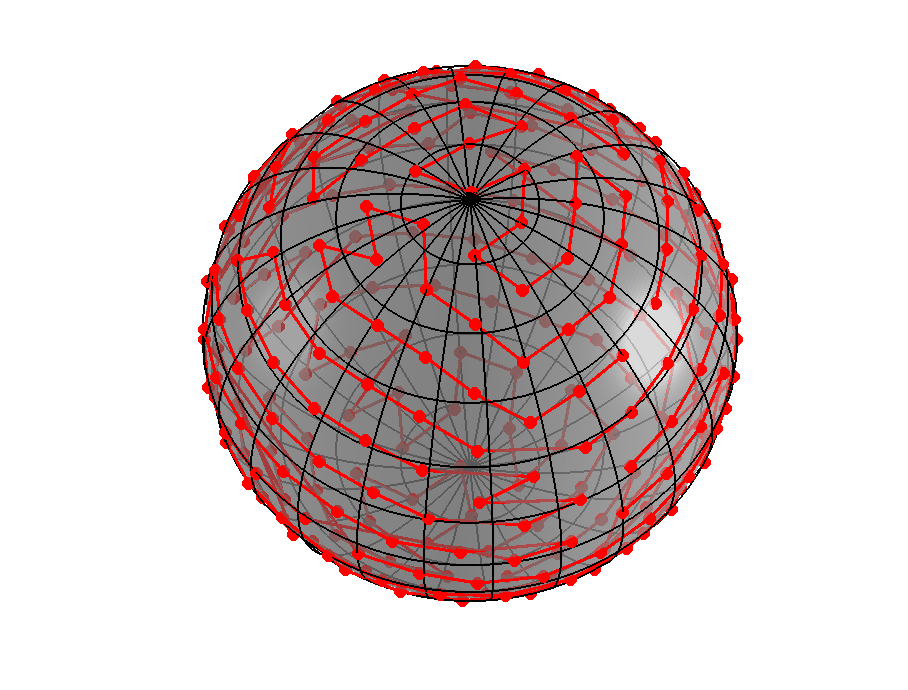
\includegraphics[width=0.49\textwidth]{Matlab/GridCoDePolar.eps}}
  \centering
  \subfigure[Constant Density Cartesian Coordinates]{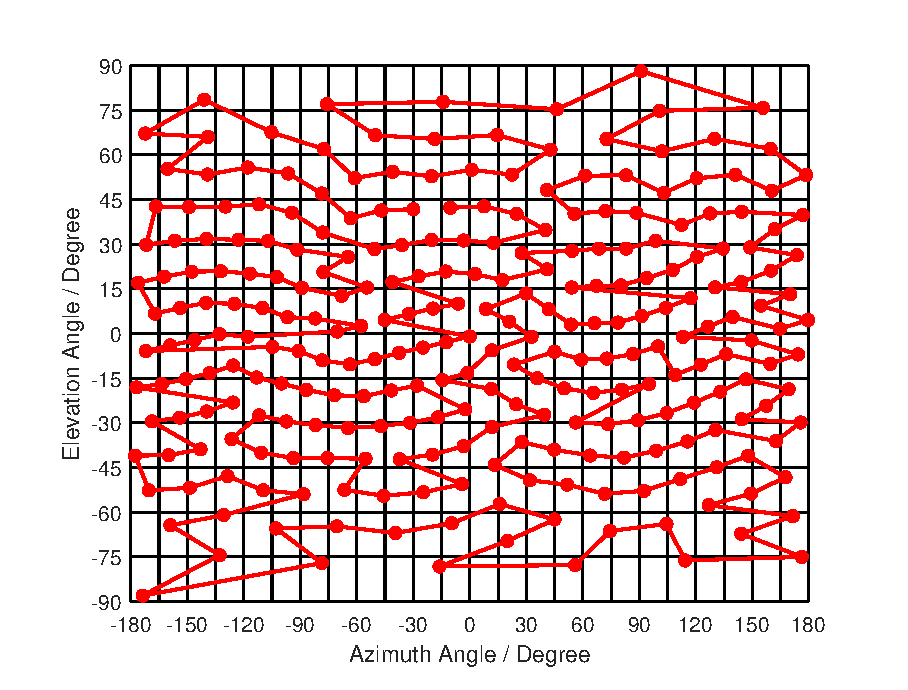
\includegraphics[width=0.49\textwidth]{Matlab/GridCoDeCart.eps}}
\caption{Different spherical sampling grids in comparison}
\label{fig:gridcomp}
\end{figure}


\begin{figure}
  \centering
  \subfigure[Two elements: Pattern]{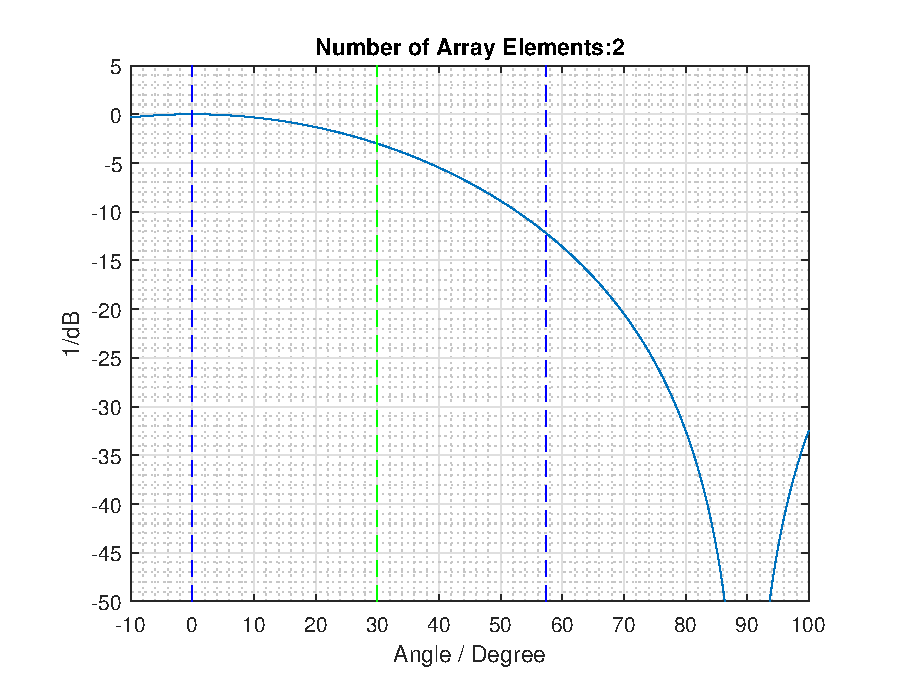
\includegraphics[width=0.45\textwidth]{Matlab/NoNumEl2.eps}}
  \centering
  \subfigure[Two elements: Mode spectra]{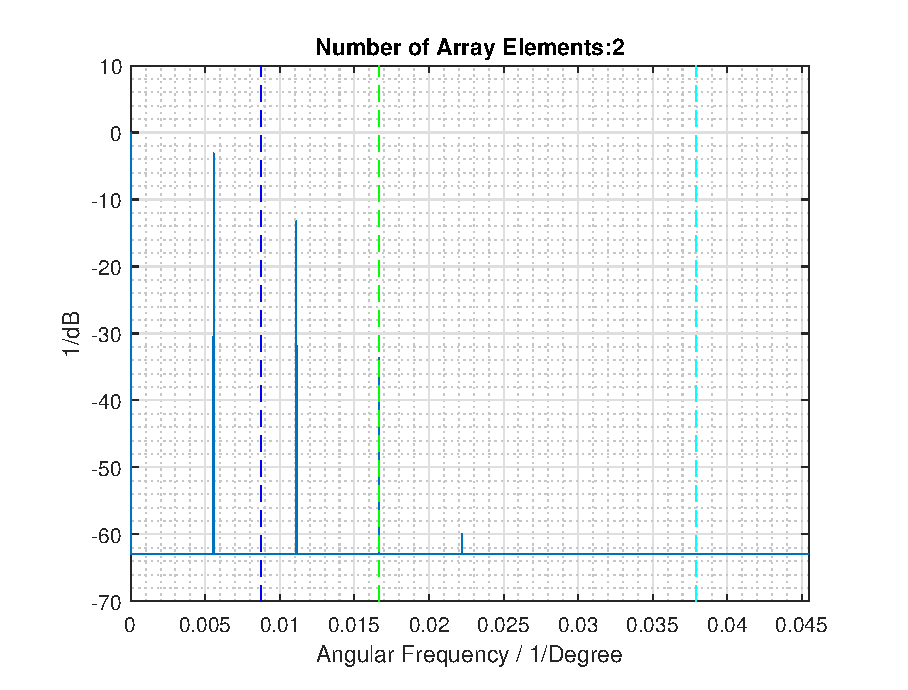
\includegraphics[width=0.45\textwidth]{Matlab/SpNumEl2.eps}}
  \centering
  \subfigure[Six elements: Pattern]{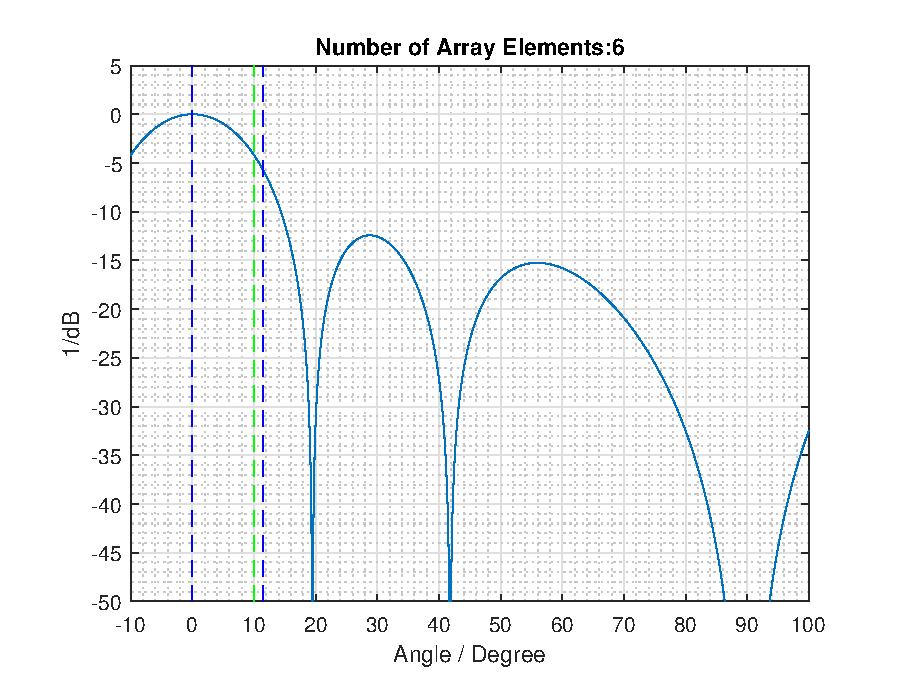
\includegraphics[width=0.45\textwidth]{Matlab/NoNumEl6.eps}}
  \centering
  \subfigure[Six elements: Mode spectra]{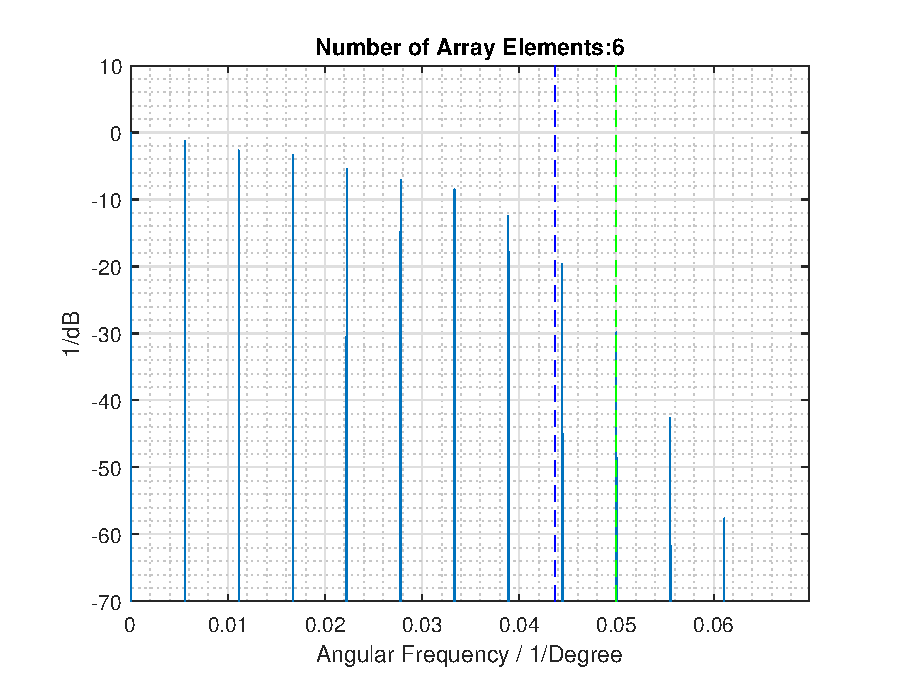
\includegraphics[width=0.45\textwidth]{Matlab/SpNumEl6.eps}}
  \centering
  \subfigure[100 elements: Pattern]{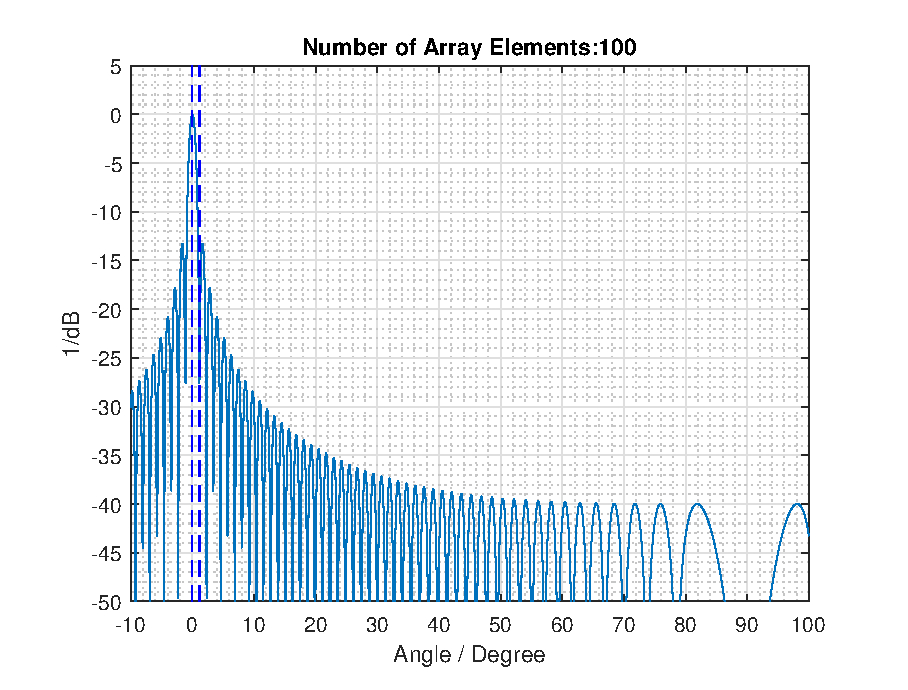
\includegraphics[width=0.45\textwidth]{Matlab/NoNumEl100.eps}}
  \centering
  \subfigure[100 elements: Mode spectra]{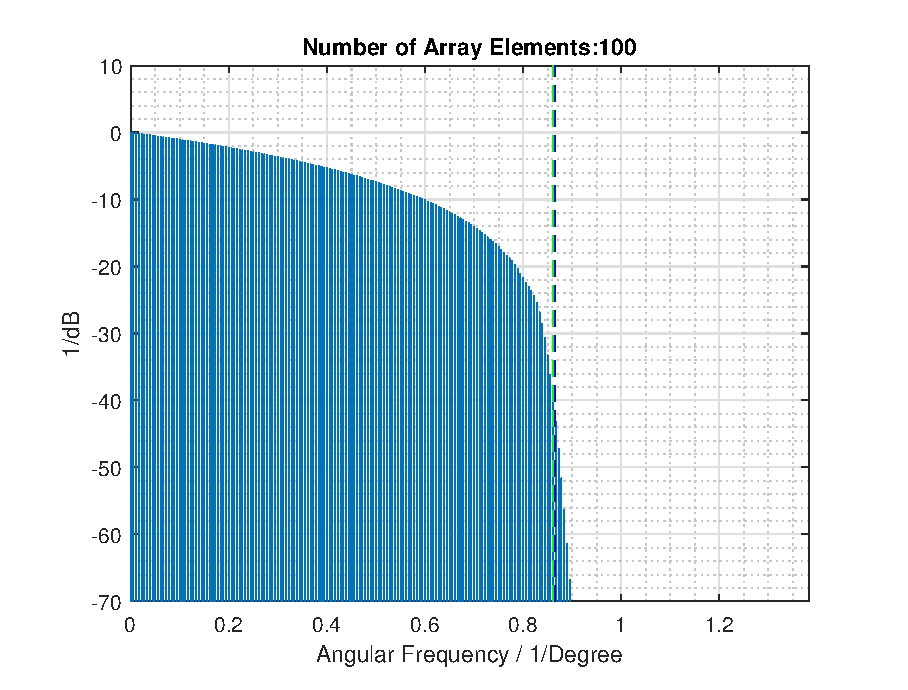
\includegraphics[width=0.45\textwidth]{Matlab/SpNumEl100.eps}}
\caption{Pattern of $N$-element $\sfrac{\lambda}{2}$-spacing}
\label{fig:evolvpattern}
\end{figure}

\begin{figure}
\centering
  \centering
  \subfigure[E-Field]{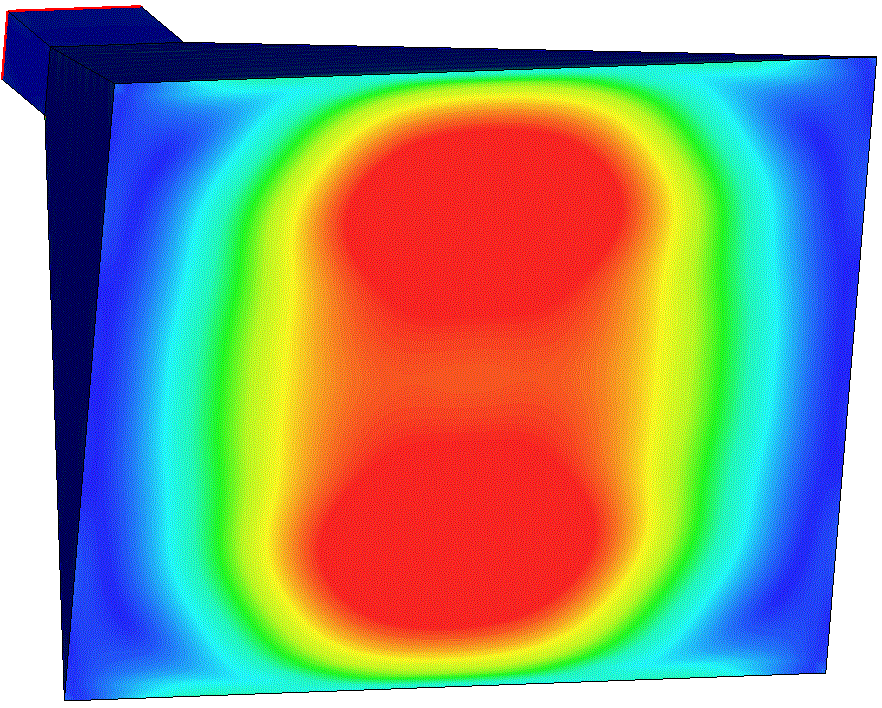
\includegraphics[width=0.49\textwidth]{horn_e_Field_FrontView.png}}
  \centering
  \subfigure[H-Field]{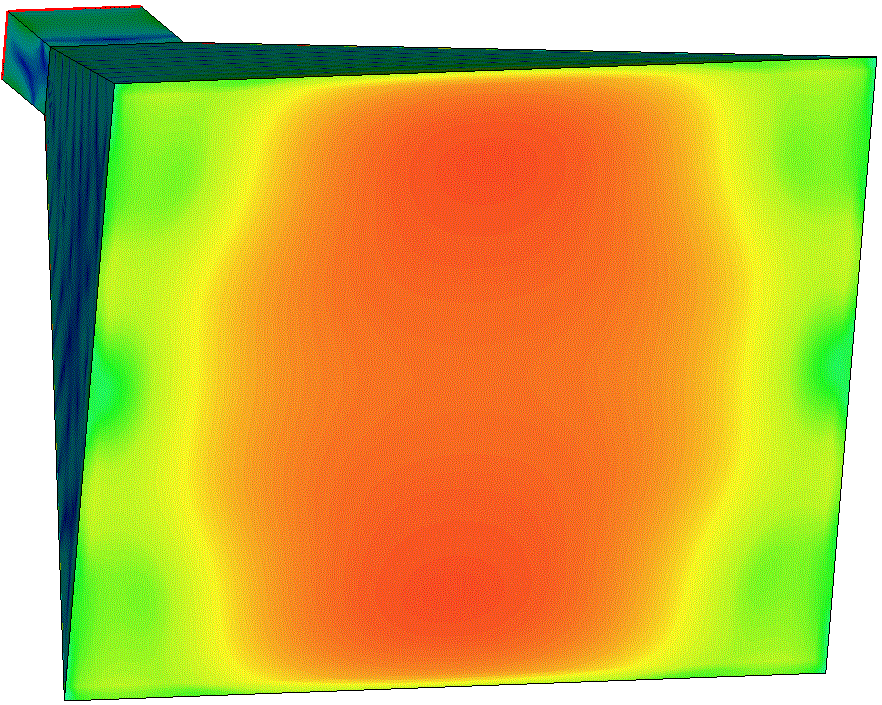
\includegraphics[width=0.49\textwidth]{horn_h_Field_FrontView.png}}
\caption{Field distribution on the aperture of a $\SI{20}{\decibel}$ \ac{SGH} at $\SI{28}{\giga\hertz}$}
\label{fig:fielddist}
\end{figure}

\begin{figure}
\centering
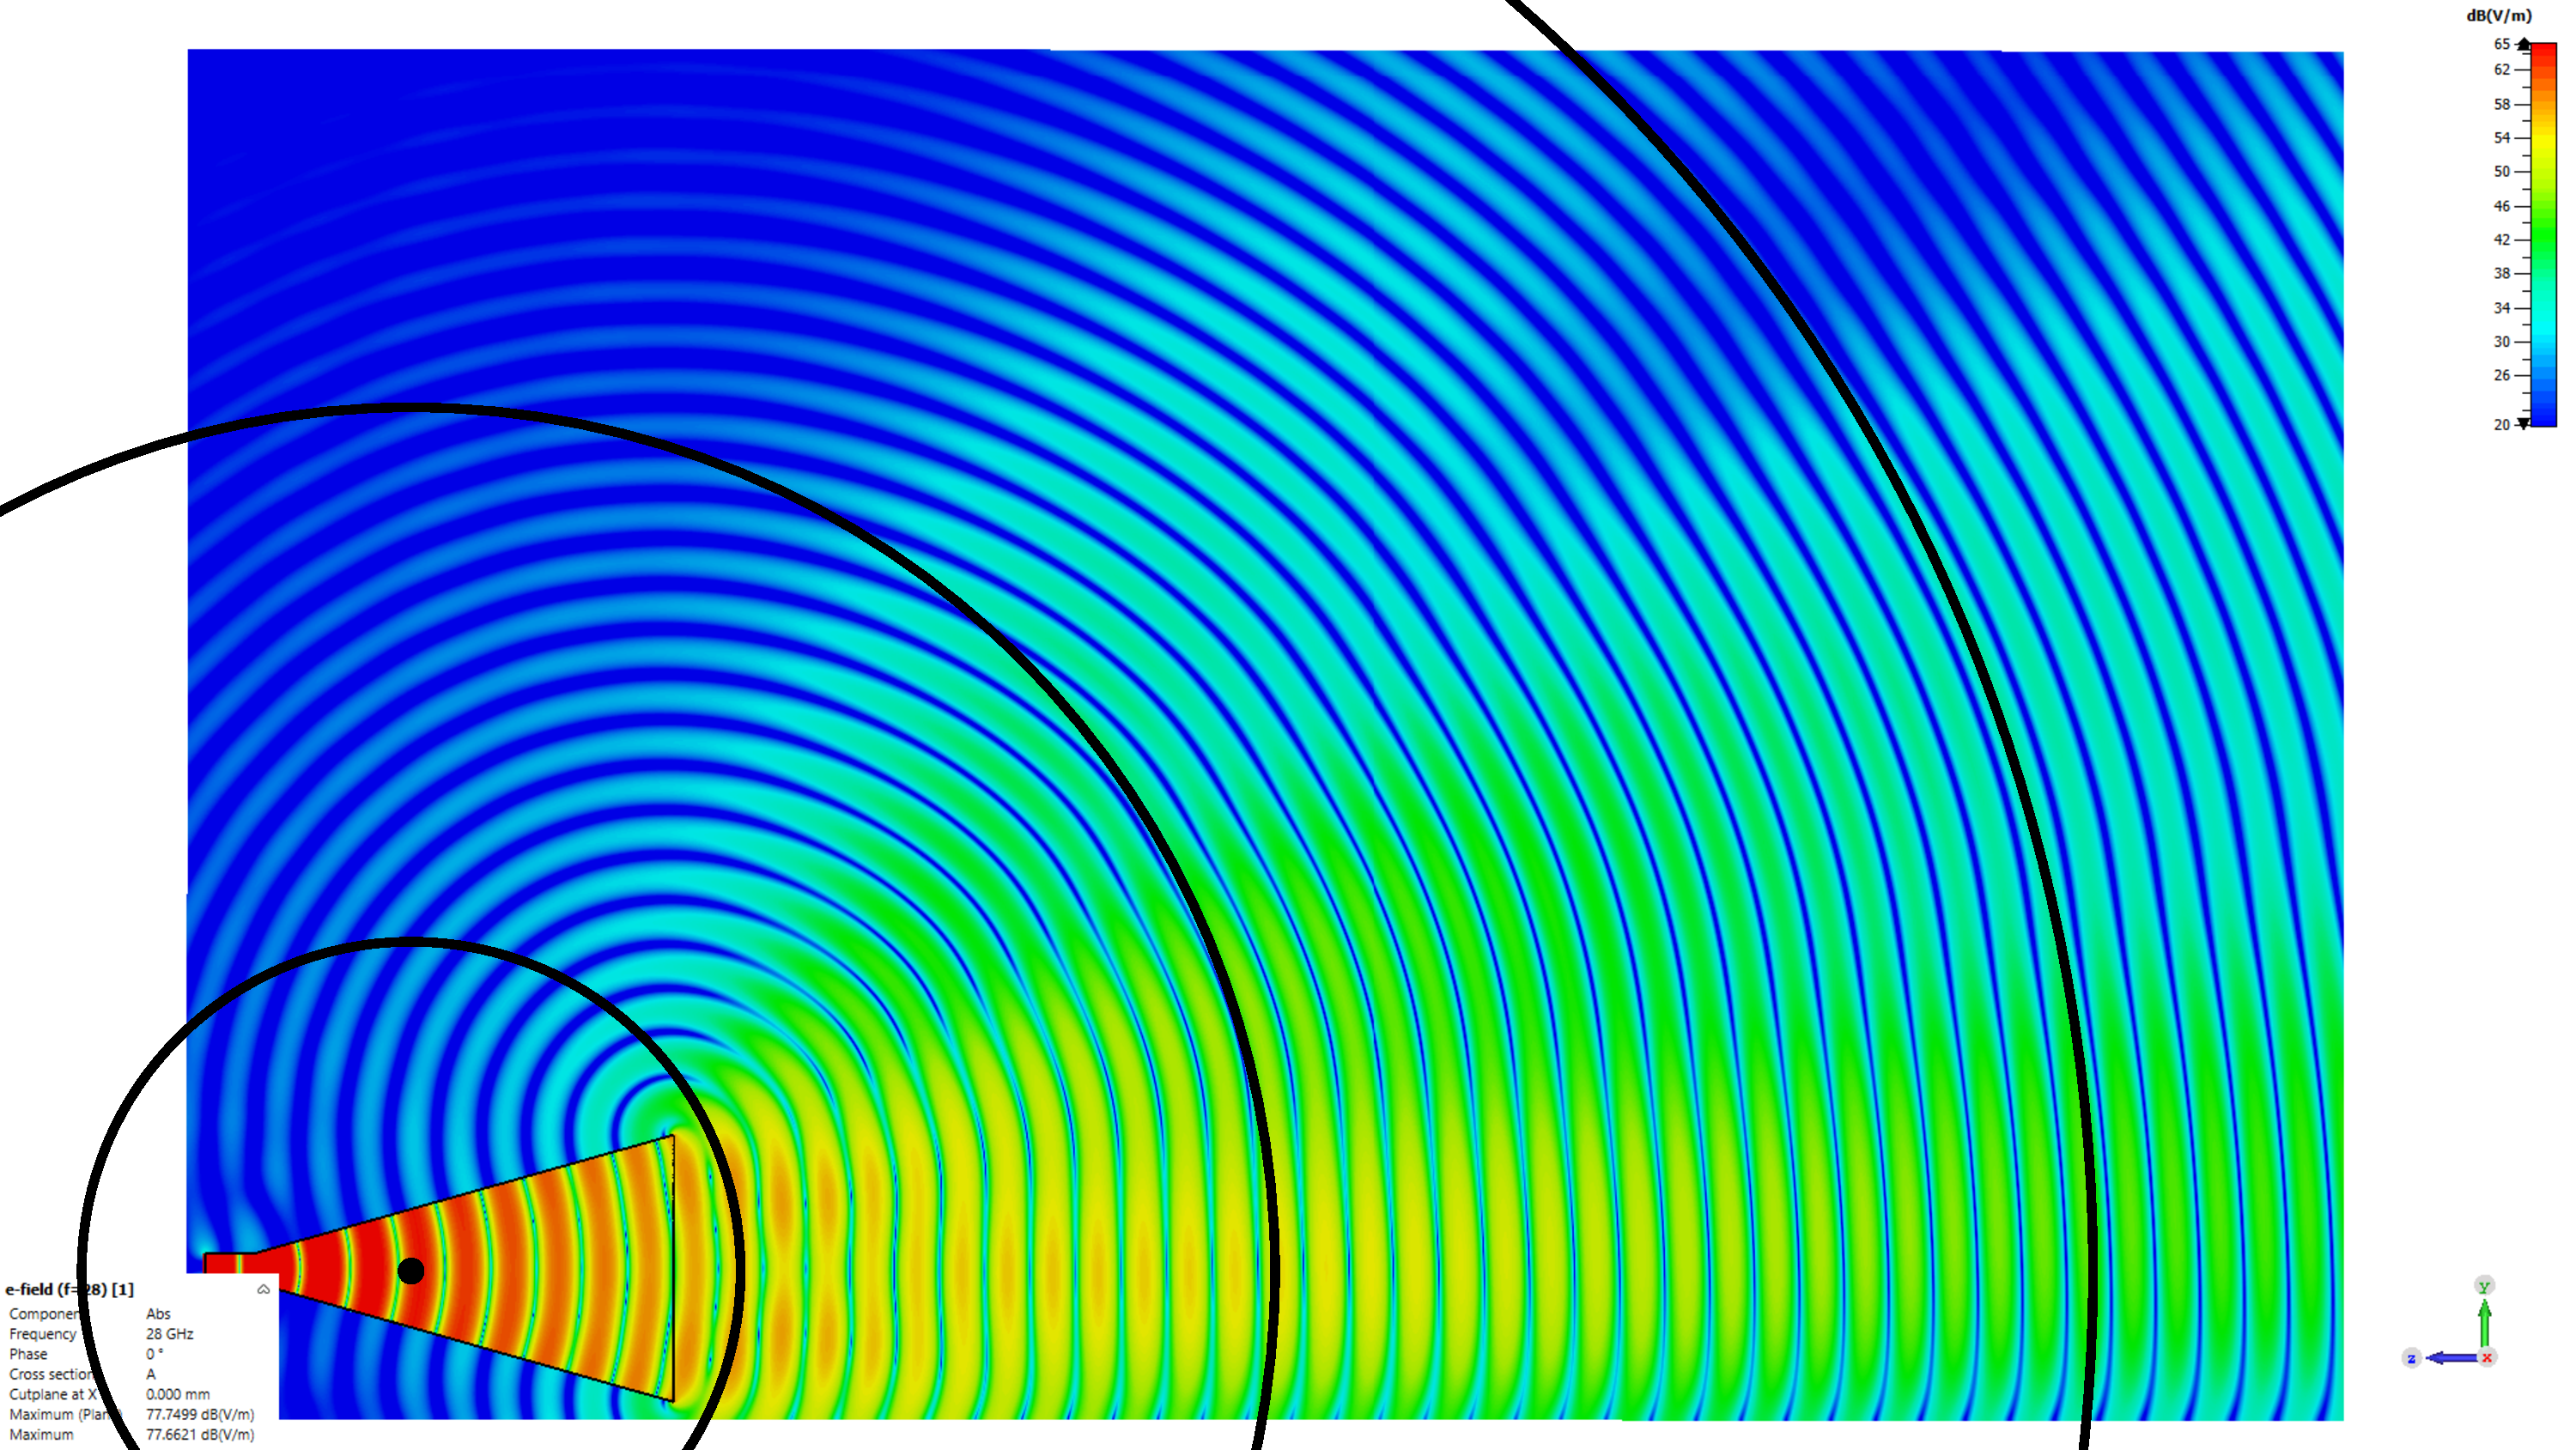
\includegraphics[width=1.5\textwidth , angle=90]{Horn-ef-Field-Region.pdf}
\caption{E-Field of a \ac{SGH} in E-Plane}
\label{fig:eplaneef}
\end{figure}
\begin{figure}
\centering
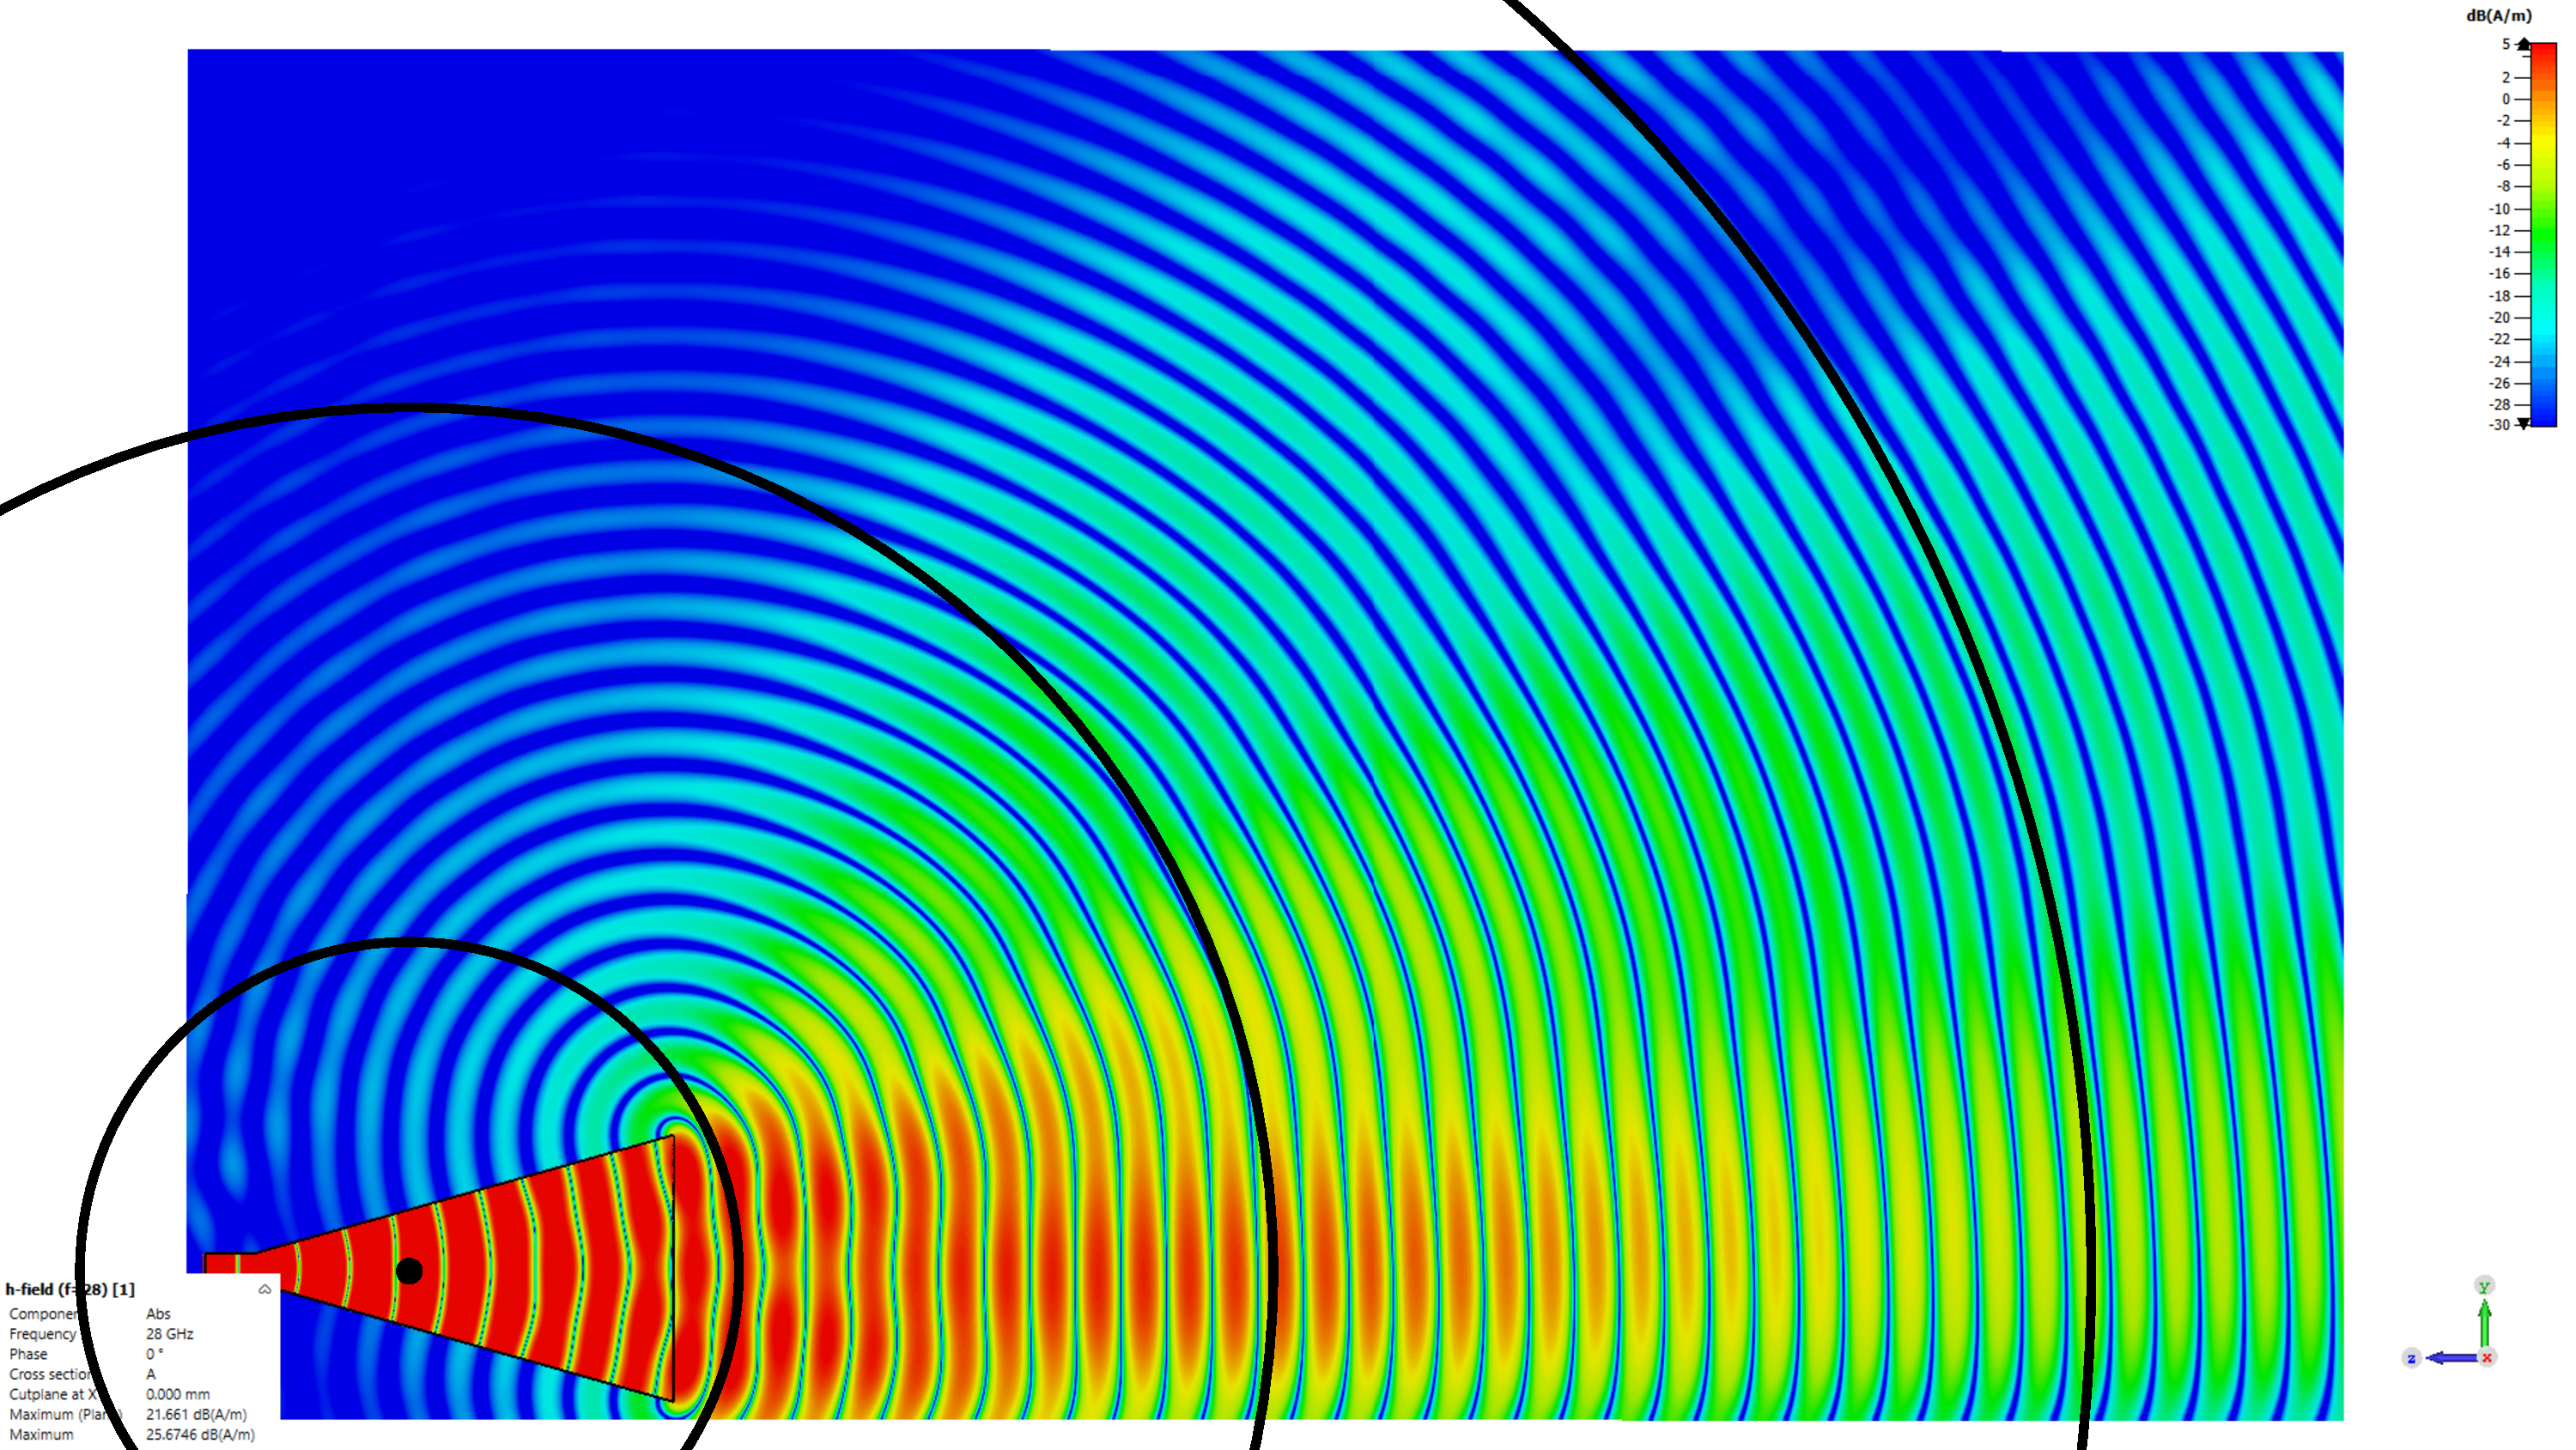
\includegraphics[width=1.5\textwidth , angle=90]{Horn-hf-Field-Region.pdf}
\caption{H-Field of a \ac{SGH} in E-Plane}
\label{fig:eplaneef}
\end{figure}

\begin{figure}
  \centering
  \subfigure[Cartesian]{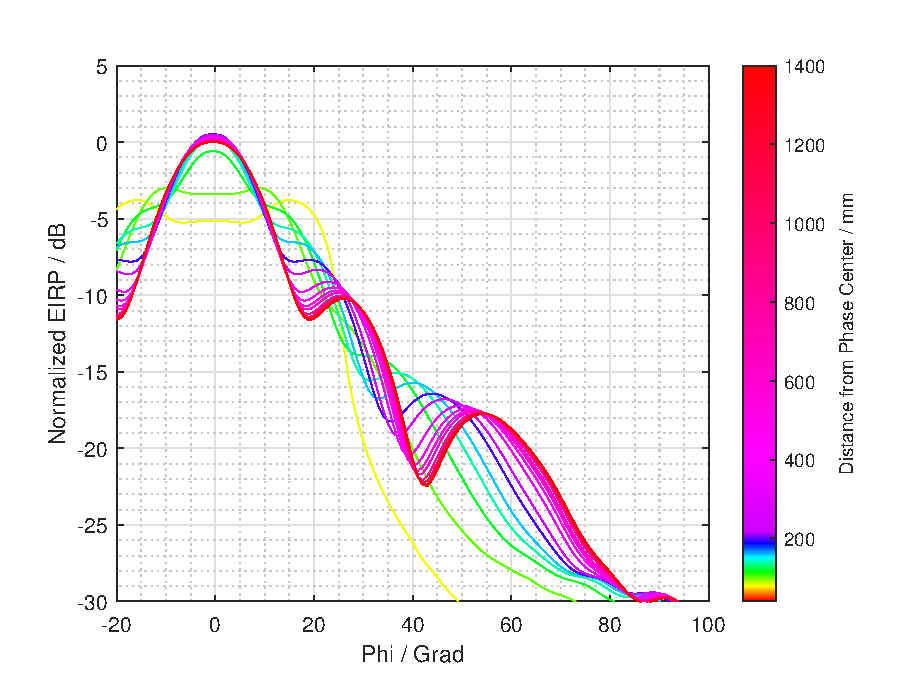
\includegraphics[width=0.8\textwidth]{Matlab/evolvePattern1.eps}}
  \centering
  \subfigure[Polar]{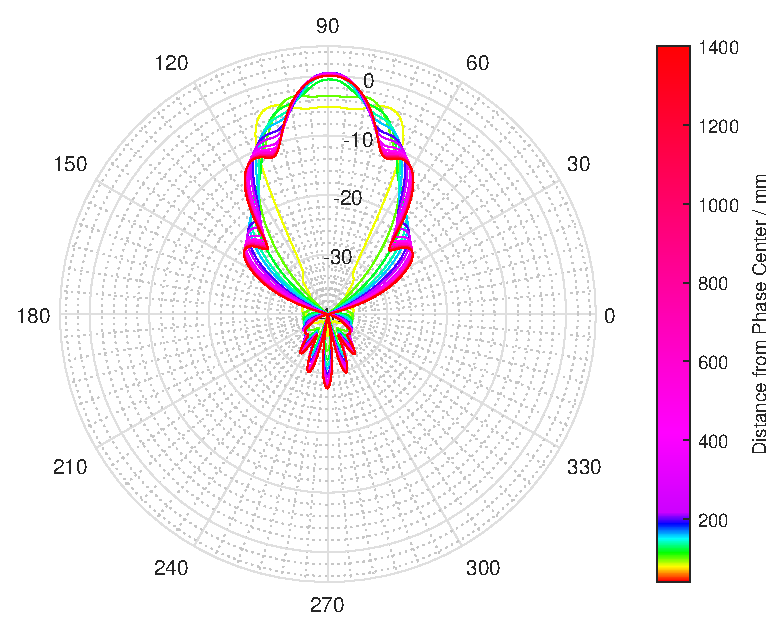
\includegraphics[width=0.8\textwidth]{Matlab/evolvePattern2.eps}}
\caption{Development of the antenna pattern in different radii}
\label{fig:devantennap}
\end{figure}